\documentclass[conference]{IEEEtran}
\IEEEoverridecommandlockouts
% The preceding line is only needed to identify funding in the first footnote. If that is unneeded, please comment it out.
\usepackage{cite}
\usepackage{amsmath,amssymb,amsfonts}
\usepackage{algorithmic}
\usepackage{graphicx}
\usepackage{textcomp}
\usepackage{xcolor}
\def\BibTeX{{\rm B\kern-.05em{\sc i\kern-.025em b}\kern-.08em
    T\kern-.1667em\lower.7ex\hbox{E}\kern-.125emX}}
\begin{document}

\title{Predicting the Average Two-Year Winning Percent and Hire Tenure of NFL Head Coach Hires: Three Approaches}

\author{\IEEEauthorblockN{Jon C. Williamson}
\IEEEauthorblockA{\textit{Dept. of Computer Science \& Engineering} \\
\textit{Texas A\&M University}\\
College Station, TX, USA \\
jonwilliamson@tamu.edu}
}

\maketitle

\begin{abstract}
This document is a model and instructions for \LaTeX.
This and the IEEEtran.cls file define the components of your paper [title, text, heads, etc.]. *CRITICAL: Do Not Use Symbols, Special Characters, Footnotes, 
or Math in Paper Title or Abstract.
\end{abstract}

\begin{IEEEkeywords}
machine learning, neural networks, prediction methods, supervised learning, unsupervised learning
\end{IEEEkeywords}

\section{Introduction}
Although the National Football League (NFL) is not publicly traded, evaluation of its teams suggests that it is worth over \$91 billion dollars \cite{b1}.  Equivalently, the average NFL franchise is worth \$2.86 billion dollars \cite{b1}. Despite these large evaluations, hiring successful head coaches is anything but repeatable in the NFL. In 2016, the median head coach tenure in position was three years \cite{b2}. Although this length is marginally better than other sports leagues \cite{b2}, comparing the average top job tenure to public sector best practice shows immense area for improvement. A publicly traded company that changed CEOs at this rate would have an extremely volatile stock price and likely decreased stock demand \cite{b3}. In this analogy, the general manager is the entire Board of Directors. Moreover, successful head coach hiring is tremendously valuable, as a differentiated NFL head coach can bring about lasting success and divisional dominance, subsequently increasing the historical importance of a franchise and improving its bottom line. A machine learning model that can increase the hit percentage of head coaching hires has the potential to add immense value to NFL franchises. This project attempts to predict two outcomes of head coach hires: the average two-year winning percent and the hire tenure, using three machine learning approaches.

\section{Literature Review}
There have been no journal publications that attempt to predict the success of NFL coaching hires through statistical learning techniques. Currently, the NFL is only beginning to implement artificial intelligence (AI) in play calling prediction \cite{b4}. Additionally, there are few papers that examine the impact of individual features on NFL head coaching success. Reference \cite{b5} used a linear regression with seven features to attempt to predict the number of wins of head coaches in their first three years in order to understand if prior NFL head coaching experience impacts success in position. This paper found that a previous head coaching experience had a negative impact on the success of new head coaches. Despite this finding, the model supported an adjusted $R^2$ of only $0.336$. This low value does not instill confidence in its findings or feature weights. Additionally, the lack of regularization and the small number of features further decrease confidence in the findings. Reference \cite{b6} reviews research in sports economics and suggests that hiring decisions made solely on playing success are unlikely to be optimal given financial (conditional) inequality among sports franchises. 

\section{Problem Formulation}
This project develops three implementations of two machine learning models. The first model attempts to predict a coach's average winning percentage in their first two years following hiring using three separate regressors. The second model attempts to predict a classification of coach tenure following hiring using three multi-class classifiers. Although the feature set and data points for these problems are largely identical, this report will analyze both models separately.

\section{Proposed Solution}

\subsection{Predicting Average Two-Year Winning Percent}
Equation \eqref{eq1} defines the calculation of average winning percentage, $p_{win}$, as a function of the number of wins, $n_{wins}$, the number of losses, $n_{losses}$, and the number of ties, $n_{ties}$, of a head coach over any interval. 

\begin{equation}
        p_{win}=\frac{n_{wins} + 0.5*n_{ties}}{n_{wins} + n_{losses} + n_{ties}}
        \label{eq1}
\end{equation}

This winning percentage is bound within $[0, 1]$. Predicting this continuous value requires regression. This project implements three regressors to attempt this prediction: 
\begin{enumerate}
  \item Linear Regression with Lasso Regularization\cite{b7}
  \item XGBoost Regressor\cite{b8}
  \item Multi-layer Perceptron Regressor\cite{b7}
\end{enumerate}

The first implementation of this model is a simple linear model with $\ell_1$ norm regularization. This project uses $\ell_1$ regularization due to its tendency to remove features from the model. The second implementation of the model is an XGBoost Regressor. This regressor uses gradient boosting to build a single predication model through the aggregation of weak learners. This project uses trees as the universal model for the weak learners. The third and final implementation of this model is through a Multi-layer Perceptron Regressor. This regressor is a basic neural network with a final regression node. It extracts features without supervision. This project utilizes extensive cross-validation to determine the optimal values for hyperparameters for each model implementation. 

This project uses root mean squared error (RMSE) as the evaluation metric for these regression models. This metric was chosen for two reasons. Firstly, its dimensions are identical to the dimensions of the prediction variable. Secondly, it punishes outliers greater than absolute error. It is important to note that the thresholds that constitute `good' and `bad' RMSE are impacted by the scale of the prediction. As a result, this project compares model RMSE against the RMSE for predicting the expected outcome in order to understand model performance. 


\subsection{Predicting Coach Tenure Class}
This project defines the tenure of a coach hire as the number of years the hired coach remains in the same position before being fired, leaving, or retiring. A model that predicts this tenure directly would require regression. This level of granularity is not necessary, as there is no meaningful difference between a coach that is in position for ten years and one that is in position for twelve years. As a result, this project maps coach tenures to four tenure classifications in order to convert this problem to a classification. Equation \eqref{eq2} shows the mapping between the coach tenure, $t$, and coach tenure classification labels, $C(t)$.
\begin{equation}
        C(t)=
        \begin{cases}
            0 &t \leq 2 		\\
            1 &2 < t \leq 4 \\
            2 &4 < t \leq 7 \\
            3 &t > 7
        \end{cases}
        \label{eq2}
\end{equation}

Equation \eqref{eq2} shows four independent coach tenure classification labels. The shortest tenure class, of one and two years, is intended to capture the worst head coach hires. The next class, of three and four years, is intended to capture coaches that are mediocre, i.e., coaches that teams would be happy to move on from but are not obligated to do so. The third coach tenure class is intended to capture successful head coaches with tenure between five and seven years. The fourth and final class is intended to capture the best coach hires in the history of the NFL, e.g., the Bill Belichick's and Don Shula's of the league.

This model seeks to predict the coaching tenure classification of head coach hires based on statistics available at the time of hiring. This project utilizes three implementations of this model:
\begin{enumerate}
  \item Logistic Regression with Lasso Regularization\cite{b7}
  \item XGBoost\cite{b8}
  \item Multi-layer Perceptron Classifier\cite{b7}
\end{enumerate}
These implementations are analogous to the three models in the previous subsection. The primary difference is that these implementations are classification models and not regression models. As with the previous model, this project utilizes extensive cross-validation to determine hyperparameter values for each implementation. This project uses weighted one-versus-rest (OVR) area under the receiver operating characteristic curve (AUROC) to measure model performance. This performance metric accounts for class imbalance by weighing the OVR AUROC scores for each class by their prevalence in the entire data set.

\section{Data Description}
This project utilizes 25 features, two description labels, and the two model outputs for each head coaching hire. The two descriptive labels are the coach name and the hire year. These labels exist only to better understand the results, and are not included in the prediction method any model. Table \ref{tab1} shows the 25 features used in each model. Abbreviations included in feature descriptions include offensive coordinator (OC), defensive coordinator (DC), and head coach (HC).

\begin{table}[htbp]
\caption{Model Feature List}
\begin{center}
\begin{tabular}{|c||l|}
\hline
\textbf{No.} & \textbf{Description} \\
\hline
\hline
1 & Age at hiring \\
\hline
2 & Number of times previously hired as head coach \\
\hline
3 & Number of years’ experience as college position coach \\
\hline
4 & Number of years’ experience as college coordinator \\
\hline
5 & Number of years’ experience as college head coach \\
\hline
6 & Number of years’ experience as NFL position coach \\
\hline
7 & Number of years’ experience as NFL coordinator \\
\hline
8 & Number of years’ experience as NFL head coach \\
\hline
9 & Demotion presence in hiring history \\
\hline
10 & During years as NFL OC, team’s avg. norm. yardage rank \\
\hline
11 & During years as NFL OC, team’s avg. norm. point rank \\
\hline
12 & During years as NFL OC, team’s avg. norm. giveaway rank \\
\hline
13 & During years as NFL DC, team’s avg. norm. yardage rank \\
\hline
14 & During years as NFL DC, team’s avg. norm. point rank \\
\hline
15 & During years as NFL DC, team’s avg. norm. turnover rank \\
\hline
16 & During years as NFL HC, team’s avg. norm. yardage differential\\
&rank \\
\hline
17 & During years as NFL HC, team’s avg. norm. point differential \\
&rank \\
\hline
18 & During years as NFL HC, team’s avg. norm. turnover ratio rank \\
\hline
19 & Hiring team’s avg. winning percent in previous two years \\
\hline
20 & Hiring team’s avg. norm. turnover ratio rank in previous two \\
&years \\
\hline
21 & Hiring team’s avg. norm. point differential rank in previous\\
& two years \\
\hline
22 & Hiring team’s avg. norm. yard differential rank in previous\\
&two years \\
\hline
23 & Hiring team’s avg. norm. divisional placement in previous two\\
&years \\
\hline
24 & Hiring team’s number of playoff appearances in previous\\
&two years \\
\hline
25 & Hiring team’s number of playoff wins in previous two years \\
\hline
\end{tabular}
\label{tab1}
\end{center}
\end{table}

Table \ref{tab1} shows that features 1 through 18 are characteristics of head coaches at time of hiring, while features 19 through 25 are characteristics of the hiring team. This distinction is essential, as resource inequality among franchises does impact team success independent of any coaching effort \cite{b6}. Moreover, this project includes these team-specific features because the models could determine profiles of successful coaches with respect to team state in order to maximize win total and coach tenure. All features are purely numeric. Only one feature, feature 9, is categorical. All other features are continuous.

Features 10 through 18 and 20 through 23 reference average normalized team ranks in different categories. For these features, the single feature value is taken as the average of the normalized ranks for all years that qualify. A single feature instance prior to averaging for these features is the forms was of $x \text{ out of }z$, where $x$ is the rank of the attribute by team out of $z$ total teams. Equation \eqref{eq3} linearly distributes the feature instance value from 1 at the best rank to 0 at the worst rank:

\begin{equation}
        f(x,z) = \frac{z-x}{z-1}
        \label{eq3}
\end{equation}

Raw data was collected by scraping pro-football-reference.com. The crawling script extracted three performance tables for all head coaches in NFL history. For any coach, these three tables detail the top-level coaching results, the team's ranks in many categories relative to the league, and the coach's career hiring record for every year in their career. 

The crawling script also extracted two performance tables for all franchises in NFL history. For any franchise, these two tables include the team's record \& ranks and playoff statistics for every season in franchise history.

A script was written to analyze the crawled data to extract the feature set and calculate the two model outputs for all coach hires in NFL history. It should be noted that this script considers interim promotions acts of coach hiring, as exceptional performance as an interim coach can lead to a non-interim promotion. 

Fig. \ref{fig1} shows the corrlation matrix among all 25 features. This matrix shows that the data is not highly correlated. The three-by-three white boxes in the matrix show that there is no correlation among features 10 through 12 and 13 through 15. Features 10 through 12 are based on team performance as an offensive coordinator, while features 13 through 15 are from performance as a defensive coordinator. No coaches in the set were both an OC and a DC prior to being hired, hence there is no correlation value among those features. 

There is some correlation among features 19 through 25. Recall that these features are characteristics of hiring teams in the two years prior to the 

\begin{figure}[htbp]
\centerline{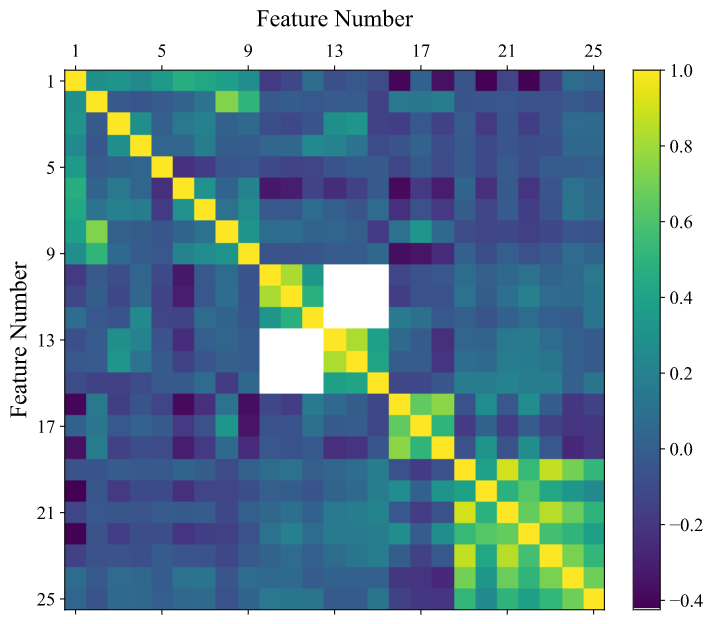
\includegraphics[width=1\linewidth]{corr.png}}
\caption{Feature correlation matrix.}
\label{fig1}
\end{figure}



\section{Results}

\section{Limitations and Future Directions}

\section{Conclusions}

\section{Ease of Use}

\subsection{Maintaining the Integrity of the Specifications}

The IEEEtran class file is used to format your paper and style the text. All margins, 
column widths, line spaces, and text fonts are prescribed; please do not 
alter them. You may note peculiarities. For example, the head margin
measures proportionately more than is customary. This measurement 
and others are deliberate, using specifications that anticipate your paper 
as one part of the entire proceedings, and not as an independent document. 
Please do not revise any of the current designations.

\section{Prepare Your Paper Before Styling}
Before you begin to format your paper, first write and save the content as a 
separate text file. Complete all content and organizational editing before 
formatting. Please note sections \ref{AA}--\ref{SCM} below for more information on 
proofreading, spelling and grammar.

Keep your text and graphic files separate until after the text has been 
formatted and styled. Do not number text heads---{\LaTeX} will do that 
for you.

\subsection{Abbreviations and Acronyms}\label{AA}
Define abbreviations and acronyms the first time they are used in the text, 
even after they have been defined in the abstract. Abbreviations such as 
IEEE, SI, MKS, CGS, ac, dc, and rms do not have to be defined. Do not use 
abbreviations in the title or heads unless they are unavoidable.

\subsection{Units}
\begin{itemize}
\item Use either SI (MKS) or CGS as primary units. (SI units are encouraged.) English units may be used as secondary units (in parentheses). An exception would be the use of English units as identifiers in trade, such as ``3.5-inch disk drive''.
\item Avoid combining SI and CGS units, such as current in amperes and magnetic field in oersteds. This often leads to confusion because equations do not balance dimensionally. If you must use mixed units, clearly state the units for each quantity that you use in an equation.
\item Do not mix complete spellings and abbreviations of units: ``Wb/m\textsuperscript{2}'' or ``webers per square meter'', not ``webers/m\textsuperscript{2}''. Spell out units when they appear in text: ``. . . a few henries'', not ``. . . a few H''.
\item Use a zero before decimal points: ``0.25'', not ``.25''. Use ``cm\textsuperscript{3}'', not ``cc''.)
\end{itemize}

\subsection{Equations}
Number equations consecutively. To make your 
equations more compact, you may use the solidus (~/~), the exp function, or 
appropriate exponents. Italicize Roman symbols for quantities and variables, 
but not Greek symbols. Use a long dash rather than a hyphen for a minus 
sign. Punctuate equations with commas or periods when they are part of a 
sentence, as in:
\begin{equation}
a+b=\gamma\label{eq}
\end{equation}

Be sure that the 
symbols in your equation have been defined before or immediately following 
the equation. Use ``\eqref{eq}'', not ``Eq.~\eqref{eq}'' or ``equation \eqref{eq}'', except at 
the beginning of a sentence: ``Equation \eqref{eq} is . . .''

\subsection{\LaTeX-Specific Advice}

Please use ``soft'' (e.g., \verb|\eqref{Eq}|) cross references instead
of ``hard'' references (e.g., \verb|(1)|). That will make it possible
to combine sections, add equations, or change the order of figures or
citations without having to go through the file line by line.

Please don't use the \verb|{eqnarray}| equation environment. Use
\verb|{align}| or \verb|{IEEEeqnarray}| instead. The \verb|{eqnarray}|
environment leaves unsightly spaces around relation symbols.

Please note that the \verb|{subequations}| environment in {\LaTeX}
will increment the main equation counter even when there are no
equation numbers displayed. If you forget that, you might write an
article in which the equation numbers skip from (17) to (20), causing
the copy editors to wonder if you've discovered a new method of
counting.

{\BibTeX} does not work by magic. It doesn't get the bibliographic
data from thin air but from .bib files. If you use {\BibTeX} to produce a
bibliography you must send the .bib files. 

{\LaTeX} can't read your mind. If you assign the same label to a
subsubsection and a table, you might find that Table I has been cross
referenced as Table IV-B3. 

{\LaTeX} does not have precognitive abilities. If you put a
\verb|\label| command before the command that updates the counter it's
supposed to be using, the label will pick up the last counter to be
cross referenced instead. In particular, a \verb|\label| command
should not go before the caption of a figure or a table.

Do not use \verb|\nonumber| inside the \verb|{array}| environment. It
will not stop equation numbers inside \verb|{array}| (there won't be
any anyway) and it might stop a wanted equation number in the
surrounding equation.

\subsection{Some Common Mistakes}\label{SCM}
\begin{itemize}
\item The word ``data'' is plural, not singular.
\item The subscript for the permeability of vacuum $\mu_{0}$, and other common scientific constants, is zero with subscript formatting, not a lowercase letter ``o''.
\item In American English, commas, semicolons, periods, question and exclamation marks are located within quotation marks only when a complete thought or name is cited, such as a title or full quotation. When quotation marks are used, instead of a bold or italic typeface, to highlight a word or phrase, punctuation should appear outside of the quotation marks. A parenthetical phrase or statement at the end of a sentence is punctuated outside of the closing parenthesis (like this). (A parenthetical sentence is punctuated within the parentheses.)
\item A graph within a graph is an ``inset'', not an ``insert''. The word alternatively is preferred to the word ``alternately'' (unless you really mean something that alternates).
\item Do not use the word ``essentially'' to mean ``approximately'' or ``effectively''.
\item In your paper title, if the words ``that uses'' can accurately replace the word ``using'', capitalize the ``u''; if not, keep using lower-cased.
\item Be aware of the different meanings of the homophones ``affect'' and ``effect'', ``complement'' and ``compliment'', ``discreet'' and ``discrete'', ``principal'' and ``principle''.
\item Do not confuse ``imply'' and ``infer''.
\item The prefix ``non'' is not a word; it should be joined to the word it modifies, usually without a hyphen.
\item There is no period after the ``et'' in the Latin abbreviation ``et al.''.
\item The abbreviation ``i.e.'' means ``that is'', and the abbreviation ``e.g.'' means ``for example''.
\end{itemize}
An excellent style manual for science writers is \cite{b7}.

\subsection{Authors and Affiliations}
\textbf{The class file is designed for, but not limited to, six authors.} A 
minimum of one author is required for all conference articles. Author names 
should be listed starting from left to right and then moving down to the 
next line. This is the author sequence that will be used in future citations 
and by indexing services. Names should not be listed in columns nor group by 
affiliation. Please keep your affiliations as succinct as possible (for 
example, do not differentiate among departments of the same organization).

\subsection{Identify the Headings}
Headings, or heads, are organizational devices that guide the reader through 
your paper. There are two types: component heads and text heads.

Component heads identify the different components of your paper and are not 
topically subordinate to each other. Examples include Acknowledgments and 
References and, for these, the correct style to use is ``Heading 5''. Use 
``figure caption'' for your Figure captions, and ``table head'' for your 
table title. Run-in heads, such as ``Abstract'', will require you to apply a 
style (in this case, italic) in addition to the style provided by the drop 
down menu to differentiate the head from the text.

Text heads organize the topics on a relational, hierarchical basis. For 
example, the paper title is the primary text head because all subsequent 
material relates and elaborates on this one topic. If there are two or more 
sub-topics, the next level head (uppercase Roman numerals) should be used 
and, conversely, if there are not at least two sub-topics, then no subheads 
should be introduced.

\subsection{Figures and Tables}
\paragraph{Positioning Figures and Tables} Place figures and tables at the top and 
bottom of columns. Avoid placing them in the middle of columns. Large 
figures and tables may span across both columns. Figure captions should be 
below the figures; table heads should appear above the tables. Insert 
figures and tables after they are cited in the text. Use the abbreviation 
``Fig.~\ref{fig}'', even at the beginning of a sentence.

\begin{table}[htbp]
\caption{Table Type Styles}
\begin{center}
\begin{tabular}{|c|c|c|c|}
\hline
\textbf{Table}&\multicolumn{3}{|c|}{\textbf{Table Column Head}} \\
\cline{2-4} 
\textbf{Head} & \textbf{\textit{Table column subhead}}& \textbf{\textit{Subhead}}& \textbf{\textit{Subhead}} \\
\hline
copy& More table copy$^{\mathrm{a}}$& &  \\
\hline
\multicolumn{4}{l}{$^{\mathrm{a}}$Sample of a Table footnote.}
\end{tabular}
\label{tab2}
\end{center}
\end{table}

\begin{figure}[htbp]
\centerline{
\includegraphics{fig1.png}}
\caption{Example of a figure caption.}
\label{fig}
\end{figure}

Figure Labels: Use 8 point Times New Roman for Figure labels. Use words 
rather than symbols or abbreviations when writing Figure axis labels to 
avoid confusing the reader. As an example, write the quantity 
``Magnetization'', or ``Magnetization, M'', not just ``M''. If including 
units in the label, present them within parentheses. Do not label axes only 
with units. In the example, write ``Magnetization (A/m)'' or ``Magnetization 
\{A[m(1)]\}'', not just ``A/m''. Do not label axes with a ratio of 
quantities and units. For example, write ``Temperature (K)'', not 
``Temperature/K''.

\section*{Acknowledgment}

The preferred spelling of the word ``acknowledgment'' in America is without 
an ``e'' after the ``g''. Avoid the stilted expression ``one of us (R. B. 
G.) thanks $\ldots$''. Instead, try ``R. B. G. thanks$\ldots$''. Put sponsor 
acknowledgments in the unnumbered footnote on the first page.

\section*{References}

Please number citations consecutively within brackets \cite{b1}. The 
sentence punctuation follows the bracket \cite{b2}. Refer simply to the reference 
number, as in \cite{b3}---do not use ``Ref. \cite{b3}'' or ``reference \cite{b3}'' except at 
the beginning of a sentence: ``Reference \cite{b3} was the first $\ldots$''

Number footnotes separately in superscripts. Place the actual footnote at 
the bottom of the column in which it was cited. Do not put footnotes in the 
abstract or reference list. Use letters for table footnotes.

Unless there are six authors or more give all authors' names; do not use 
``et al.''. Papers that have not been published, even if they have been 
submitted for publication, should be cited as ``unpublished'' \cite{b4}. Papers 
that have been accepted for publication should be cited as ``in press'' \cite{b5}. 
Capitalize only the first word in a paper title, except for proper nouns and 
element symbols.

For papers published in translation journals, please give the English 
citation first, followed by the original foreign-language citation \cite{b6}.

\begin{thebibliography}{00}
\bibitem{b1} T. Barrabi, ``What is the NFL worth? Revenue, team values and other financial facts,'' Fox Business. https://www.foxbusiness.com/sports/nfl-worthrevenue-team-values (accessed Oct. 26, 2020)
\bibitem{b2} C. Gaines, ``NFL head coaches have good job security when compared to other major sports leagues,'' Business Insider. https://www.businessinsider.com/coaches-managers-tenure-nfl-mlb-nba-nhl-premier-league-2016-12 (accessed Oct. 26, 2020)
\bibitem{b3} ``How does a change in CEO impact stock price?,'' Investopedia. https://www.investopedia.com/ask/answers/010815/how-does-change-ceo-impact-stock-price.asp (accessed Nov. 18, 2020)
\bibitem{b4} ``Using machine learning to peek inside the minds of NFL coaches,'' DataRobot. https://www.datarobot.com/blog/using-machine-learning-to-peek-inside-the-minds-of-nfl-coaches/ (accessed Oct. 26, 2020)
\bibitem{b5} M. Roach, ``Does prior NFL head coaching experience improve team performance?,'' in Journal of Sport Management, vol. 30, no. 3, pp. 298-311.
\bibitem{b6} D. Mielke, ``Coaching experience, playing experience, and coaching tenure: a commentary,'' in International Journal of Sports Science \& Coaching, vol. 2, no. 2, pp. 117-118.
\bibitem{b7} Pedregosa et al., ``Scikit-learn: machine learning in Python,'' in Journal of Machine Learning Research, vol. 12, pp.2825-2830.
\bibitem{b8} T. Chen, and C. Guestrin, ``XGBoost: a scalable tree boosting system,'' in KDD '16: Proceedings of the 22nd ACM SIGKDD International Conference on Knowledge Discovery and Data Mining, pp.785-794.
\end{thebibliography}
\vspace{12pt}
\color{red}
IEEE conference templates contain guidance text for composing and formatting conference papers. Please ensure that all template text is removed from your conference paper prior to submission to the conference. Failure to remove the template text from your paper may result in your paper not being published.

\end{document}
